\chapter{Implementing Clustering in \atwo{}}
\label{chap:implementation}
In this section, we describe problems we encounter and implementation specific considerations we make when implementing our design in \atwo{}. We begin by outlining the modifications we make to the \atwo{} system to accommodate the clustering implementation. Next, we explain implementation specific details regarding the Clustering and Demote services. Last, we discuss the consequences of some implementation details, and how they affect performance and fault tolerance. 

\section{Modifications to \atwo{}}
We make several changes to the architecture of the \atwo{} system, in \cref{fig:a2-architecture} we highlight the architectural additions we have made to the \atwo{} system in \cref{fig:a2-architecture}; we have added a Cluster module in the Synchrotron kernel and the Demote and Clustering services in the \atwo{} layer. The bottom layer, device drivers, is not part of this thesis. However, we modified and added code in the other layers to implement clustering.

The Cluster module of the Synchrotron layer handles the low-level details of channel hopping and dynamic assignment of initiators. Also, we implement the Clustering service which elects the CHs, announces them to the network, and lets every regular node select a CH to join using the Join service from the \atwo{} layer. We also implement the Demote service which runs after all clusters have run the Join service, it demotes CHs that have fewer nodes than the parameter \emph{minimum cluster size}. Finally, we make some slight modifications to the application layer to implement forwarding during CH rounds.

\begin{figure}[bt]
    \centering
    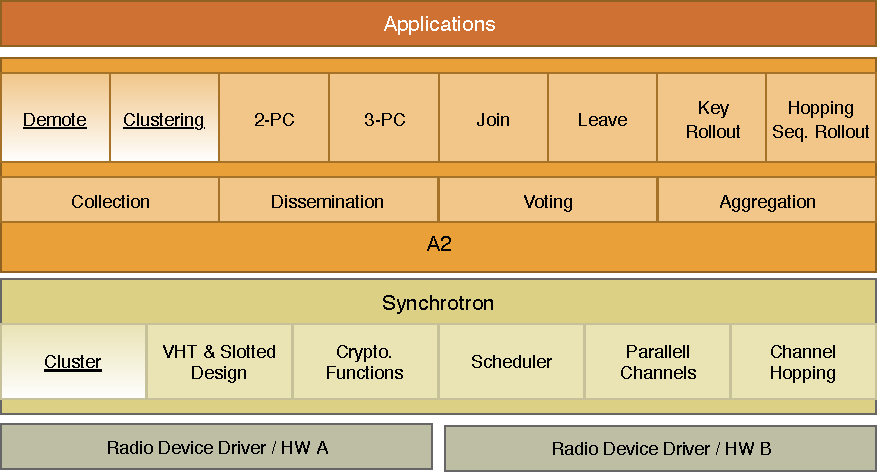
\includegraphics[width=0.7\textwidth]{figure/architecture.pdf}
    \caption{\textbf{Layered system architecture of \atwo{} \cite{a2-introduction-paper}.} Shows the placement of the Cluster and Demote services. The Cluster module in Synchrotron handles per-cluster channel hopping and dynamic assignment of initiators. The Clustering and Demote services in \atwo{} contains the logic for electing and demoting cluster heads respectively.}
    \label{fig:a2-architecture}
\end{figure}


\subsection{Flags Field for Cluster Heads}
To separate CH rounds from cluster rounds the nodes switch back and forth between intra- and inter-cluster communication every other round. Doing this means CHs are switching back and forth between different indices in the flags field as displayed in \cref{fig:flags-field-for-cluster-heads}. The Clustering service sets the flag indices used by CHs during CH rounds, and the Join service sets the flag indices used during cluster rounds. During CH rounds the CHs use the same procedure for calculating completion as during cluster rounds. However, their index in the flags field corresponds to their index in the CH list, and the length of the CH list determines the length of the flags field.

\begin{figure}[bt]
    \centering
    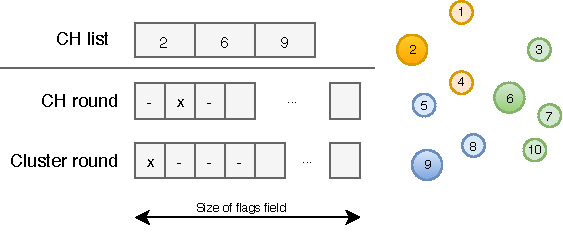
\includegraphics{figure/CH-changes-flag-index.pdf}
    \caption{
    The network on the right has elected the cluster heads in the CH list. Shown here is how Node 6 uses the flags field during CH and cluster rounds. The symbol 'x' represents the index which Node 6 uses as its flag, and the symbol '-' represents flag indices which are in use by other nodes. An empty box indicates that the index is not used. In the CH-round CHs uses the index from the CH-List. During a cluster round each CH will be an initiator and use index 0.}
    \label{fig:flags-field-for-cluster-heads}
\end{figure}

\subsection{Separating Communication Between Clusters}
\label{subsec:separating-the-clusters}
We separate the clusters in two different ways. First, we use a modified version of the channel hopping in \atwo{}. The original \atwo{} implementation hops between radio channels in two different ways as outlined in \cref{subsec-frequency-agility}. In our implementation, we separate the clusters into different channels. \atwo{}'s parallel channels functionality is deactivated since one cluster should not be large enough to interfere with its communication. The nodes still follow the original hopping sequence but offset the channel number by the \textit{cluster-index}, determined during the Clustering service. The cluster-index is unique, deterministic and since it is an index the numbers are sequential which makes it ideal to use for this purpose.

Second, each node includes its cluster ID in the packet header; if a node receives a packet from another cluster, the node discards that packet; nodes do not check this condition during CH rounds. Consequently, since all packets are slightly different in CH rounds, the constructive interference used by \atwo{} in the completion phase does not work during CH rounds.

\subsection{Forwarders During Cluster Head Rounds}
Since the HEED algorithm aims to elect non-overlapping cluster-heads, the cluster heads require assistance to communicate. Therefore, during CH-rounds all non-CH nodes act as forwarders. We implement the forwarders by letting all nodes run the Max application as usual but with the modification that non-CH nodes suggest 0 as their maximum value which is always overwritten by the CHs max value.


\subsection{Initiating Communication in a Clustered Network}
\label{subsec:implementation_the-initiator}
In our implementation, there are three different types of communication in which the initiator is different, as shown in \cref{fig:initiator-example}. First, when either the Clustering service or the Demote service is running, the network is using a single preconfigured node as the initiator. Second, during cluster rounds, each CH acts as the initiator in its cluster. Third, during CH rounds the first CH in the CH list is the initiator.

\newcommand{\rulesep}{\unskip\ \vrule\ }
\begin{figure}
\centering

\begin{subfigure}[b]{1\textwidth}
\centering
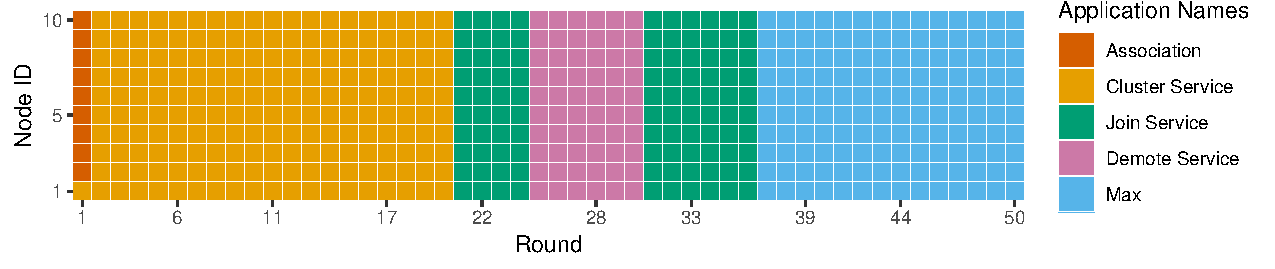
\includegraphics[width=0.75\textwidth]{figure/initiator-example/application_map.pdf}
\caption{The first 50 rounds for a network with 10 nodes, and which application each node is running. Node 1 is the initiator and thus runs the Clustering service in round 1 while the rest of the nodes associates with it.}
\end{subfigure}\quad

\begin{subfigure}[b]{1\textwidth}
\centering
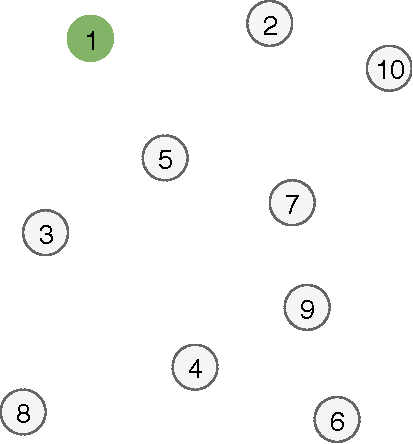
\includegraphics[width=.2\textwidth]{figure/initiator-example/location-map-proconf.pdf}\quad
\quad
\rulesep
\quad
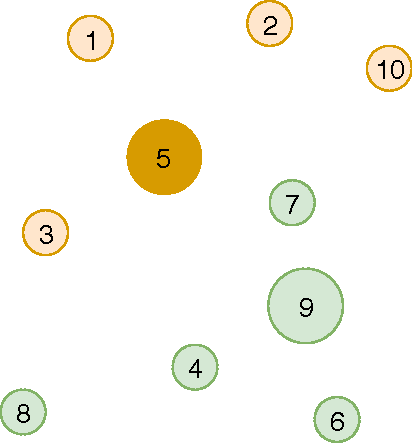
\includegraphics[width=.2\textwidth]{figure/initiator-example/location-map-ch-round.pdf}\quad
\quad
\rulesep
\quad
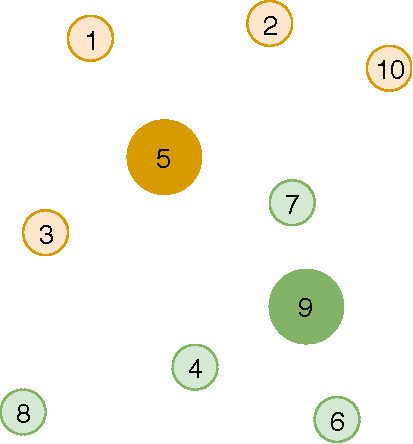
\includegraphics[width=.2\textwidth]{figure/initiator-example/location-map-cluster-round.pdf}

\caption{Locations of the ten nodes showing three different initiator setups. Node 1 is initiator rounds 1-20 and 25-30. Nodes 5 and 9 are initiators in rounds 21-24, 31-36 and every cluster (odd) round in the interval 37-50. Node 5 is the initiator in every CH (even) round in the interval 37-50.}
\label{fig:initiator-example}
\end{subfigure}

\caption{An example network and its application map. Showing which applications the network executed, and which nodes are initiators during the different phases.}

\end{figure}

Switching the initiator between different nodes introduce problems. Namely, the network can end up in a state where none of the nodes considers themselves initiator, which means every node in the network is stuck associating indefinitely. Two scenarios can occur.

First, if the CH with the lowest ID loses connection to the network, there will be no initiator during CH rounds. If that happens, no CH rounds will be executed by the network until after it has performed a re-clustering.

Second, a scenario which can occur that makes all nodes associate indefinitely.

\begin{enumerate}
    \item The preconfigured initiator node, $p$ loses connection with the network during a cluster round, when it does not consider itself initiator.
    \item The next scheduling of the Clustering service happens before $p$ can associate with the network again.
    \item In the Clustering service all nodes wait for packets from $p$, but since $p$ is associating they never receive any packets.
\end{enumerate}


\subsection{Interaction Between Services}
\label{subsec:interaction-between-services}
In this thesis, we implement two different services: the Clustering service and the Demote service. Furthermore, we use the Join service, provided by \atwo{}, within the clusters to get a consistent membership. However, for the clustering process to succeed, they have to be run in a specific order. First, the Clustering service needs to be run and converge on a set of CHs. Following that, the network executes the Join service within each cluster, allowing each CH to learn how many nodes have decided to join its cluster. Then the Demote service executes, during which CHs demote themselves if they have too few nodes in their cluster. When the network has completed the Demote service, it reruns the Join service since some clusters might have demoted themselves; the network needs to make sure that any node that changed cluster is picked up by a new cluster. At this point the clustering process is complete, and the intended operation of the network can continue.


\section{The Clustering Service}
In this section, we explain implementation specific details that are related to the Clustering service. We go into detail about the packet payload and what information we transmit from a node and why; we also describe challenges we face due to not having completion flags. Finally, we explain a Catch-up mechanism we implement in the Clustering service to handle nodes joining the network during the clustering process.

\subsection{The Clustering Service Packet Payload}
As mentioned in the design chapter, nodes running the Clustering service exchanges information to inform the network of how many CHs have announced themselves. In this section, we describe the payload of the Clustering service packet.

The content of the Clustering service packet payload is summarised in \cref{table:cluster-service-packet}. The transmitting node's ID is used in the Clustering service to count the number of packets received from a node. The consecutive cluster rounds is a counter of how many rounds has elapsed since the Clustering service started to run; we use this parameter in the Catch-up mechanism, which we explain in \cref{subsec:catch-up-mechanism}. The last entry is the CH list, which uses three bytes of space per entry. The list has a maximum size of 90 bytes, allowing a maximum of 30 CHs. Each entry in the CH list contains the CH's ID; the hop count to it; and its status, which is either \emph{Tentative} or \emph{Final}. 

The packet's payload size is restricted by the maximum packet size of the IEEE 802.15.4 standard, which is 127 bytes \cite{IEEE-802-15-4}. It is restricted further by the \atwo{} header size and data added in the link layer, giving us a maximum of 112 bytes for the payload size. As can be seen in \cref{table:cluster-service-packet}, we leave 19 bytes in the packet since some features which we are not using in \atwo{} take up space in the packet header, we do not want the Clustering service to break when other features of the \atwo{} system are activated.


\begin{table}[bt]
\centering
\caption{The parameters and their sizes in the Clustering service packet payload.}
\label{table:cluster-service-packet}
\begin{tabular}{|l|l|}
\hline
\textbf{Name}               & \textbf{Size(bytes)} \\ \hline
Source ID                   & $1$                    \\
Consecutive cluster rounds  & $1$                    \\
Cluster head count          & $1$                    \\
Cluster head list           & $3*30=90$              \\ \hline
\textbf{Total}              & \textbf{93}          \\ \hline
\end{tabular}
\end{table}

\subsection{The Catch-up Mechanism}
\label{subsec:catch-up-mechanism}
The last action a node performs in a round is to double their probability to announce itself as tentative CH. However, a problem can occur if a node associates with the network during the execution of the Clustering service. Specifically, its probability to announce itself as CH, $CH_{prob}$, will have fallen behind compared to other nodes; this is most noticeable when the network has recently started, during the initial association of all nodes. For example, nodes associating with the initiator in round one randomises their initial $CH_{prob}$ in round two. However, in round two the initiator has already doubled its own $CH_{prob}$ once.

As a remedy, we implemented a \textit{Catch-up mechanism}. In the Clustering service's packet payload, we attach the number of rounds the Clustering service has executed, which a node saves once received. At the beginning of a round, all nodes that have received a value for this variable increments it. The counter describes the number of times each node's initial $CH_{prob}$ should have doubled since the start of the Clustering service. An advantage remains for nodes already part of the network or the ones which join earlier in the service, since they have had more chances to announce themselves as CH. However, as \cref{tab:prob-no-catchup} and \cref{tab:prob-catchup} show, this advantage is very small.

\begin{table}[bt]
\centering
\caption{Probability that a node has announced itself as CH in a specific round without the Catch-up mechanism.}
\label{tab:prob-no-catchup}
\begin{tabular}{|c|c|c|cccccc|}
\hline
\textbf{Round(r)} & \textbf{$CH_{Prob}$} & \multicolumn{7}{c|}{\textbf{Cumulative probability starting at round r}}                                                                                       \\ \hline
1                 & 0.005                & 0.005 &                            &                            &                            &                            &                            &       \\ \cline{1-4}
2                 & 0.010                & 0.015 & \multicolumn{1}{c|}{0.005} &                            &                            &                            &                            &       \\ \cline{1-5}
3                 & 0.020                & 0.035 & \multicolumn{1}{c|}{0.015} & \multicolumn{1}{c|}{0.005} &                            &                            &                            &       \\ \cline{1-6}
4                 & 0.040                & 0.073 & \multicolumn{1}{c|}{0.035} & \multicolumn{1}{c|}{0.015} & \multicolumn{1}{c|}{0.005} &                            &                            &       \\ \cline{1-7}
5                 & 0.080                & 0.147 & \multicolumn{1}{c|}{0.73}  & \multicolumn{1}{c|}{0.035} & \multicolumn{1}{c|}{0.015} & \multicolumn{1}{c|}{0.005} &                            &       \\ \cline{1-8}
6                 & 0.160                & 0.284 & \multicolumn{1}{c|}{0.147} & \multicolumn{1}{c|}{0.073} & \multicolumn{1}{c|}{0.035} & \multicolumn{1}{c|}{0.015} & \multicolumn{1}{c|}{0.005} &       \\ \hline
\textbf{7}                 & \textbf{0.320}                & \textbf{0.513} & \multicolumn{1}{c|}{\textbf{0.284}} & \multicolumn{1}{c|}{\textbf{0.147}} & \multicolumn{1}{c|}{\textbf{0.073}} & \multicolumn{1}{c|}{\textbf{0.035}} & \multicolumn{1}{c|}{\textbf{0.015}} & \textbf{0.005} \\ \hline
\end{tabular}
\end{table}

    
\begin{table}[bt]
\centering
\caption{Probability that a node has announced itself as CH in a specific round with the Catch-up mechanism.}
\label{tab:prob-catchup}
\begin{tabular}{|c|c|c|cccccc|}
\hline
\textbf{Round(r)} & \textbf{$CH_{Prob}$} & \multicolumn{7}{c|}{\textbf{Cumulative probability starting at round r}}                                                                                       \\ \hline
1                 & 0.005                & 0.005 &                            &                            &                            &                            &                            &       \\ \cline{1-4}
2                 & 0.010                & 0.015 & \multicolumn{1}{c|}{0.010} &                            &                            &                            &                            &       \\ \cline{1-5}
3                 & 0.020                & 0.035 & \multicolumn{1}{c|}{0.030} & \multicolumn{1}{c|}{0.020} &                            &                            &                            &       \\ \cline{1-6}
4                 & 0.040                & 0.073 & \multicolumn{1}{c|}{0.069} & \multicolumn{1}{c|}{0.060} & \multicolumn{1}{c|}{0.040} &                            &                            &       \\ \cline{1-7}
5                 & 0.080                & 0.147 & \multicolumn{1}{c|}{0.143} & \multicolumn{1}{c|}{0.134} & \multicolumn{1}{c|}{0.117} & \multicolumn{1}{c|}{0.080} &                            &       \\ \cline{1-8}
6                 & 0.160                & 0.284 & \multicolumn{1}{c|}{0.280} & \multicolumn{1}{c|}{0.273} & \multicolumn{1}{c|}{0.258} & \multicolumn{1}{c|}{0.227} & \multicolumn{1}{c|}{0.160} &       \\ \hline
\textbf{7}                 & \textbf{0.320}                & \textbf{0.513} & \multicolumn{1}{c|}{\textbf{0.511}} & \multicolumn{1}{c|}{\textbf{0.506}} & \multicolumn{1}{c|}{\textbf{0.496}} & \multicolumn{1}{c|}{\textbf{0.474}} & \multicolumn{1}{c|}{\textbf{0.429}} & \textbf{0.320} \\ \hline
\end{tabular}
\end{table}


To motivate the usefulness of the Catch-up mechanism, we present the probability that a node has announced itself as CH at round $r$ without the Catch-up mechanism in \cref{tab:prob-no-catchup} and with the Catch-up mechanism in \cref{tab:prob-catchup}. For example, if we want to see the probability that a node which associated with the network round 3 has announced itself as CH in round 6 with the Catch-up mechanism. We look at \cref{tab:prob-catchup} for the column that has its first value in round 3 and in that column look at the value for round 6, which is 0.273.

Since the probability of a node announcing itself as CH in any round is independent, we can describe a function $P(r)$ for a node's cumulative probability to have announced itself as CH at round $r$, shown in \cref{eq:catchup-mechanism}. Let $CH_{prob}$ be the starting probability of a node and $b$ the round where a node $n$ associates with the network and starts to run the Clustering service. 

\begin{equation}
\label{eq:catchup-mechanism}
P(r) = 1 - \prod_{i = b}^r (1 - 2^i*CH_{Prob}).   
\end{equation}

Looking at \cref{tab:prob-no-catchup} and \cref{tab:prob-catchup}, where we set $CH_{prob} = 0.005$ as the initial probability, the most interesting data points are the two bottom rows, emphasised in bold. Without the Catch-up mechanism, there is a significant difference in the cumulative probability that a node has announced itself as CH. However, with the Catch-up mechanism, the difference is minimal except for in the most extreme case when a node starts at round seven, compared to a node that started at round one. A specific example shows that when we do not use the Catch-up mechanism a node that starts the Clustering service at round three will at round seven have a $0.513 - 0.147 \approx 38$ percentage points less chance of having announced itself as CH compared to a node that started at round one. However, with the Catch-up mechanism the difference is only $0.513 - 0.506 \approx 0.7$ percentage points. The same pattern can be seen for other starting points as well, giving a clear motivation that the Catch-up mechanism is useful.


\subsection{The Demote Service}
The Demote service is responsible for removing CHs that are considered suboptimal. It demotes all CHs which have fewer nodes in their cluster than the parameter \emph{minimum cluster size}.

The Demote service behaves similarly to the Clustering service; each CH decides to demote itself locally. The service is then run for some number of rounds to ensure that the information spreads to the whole network. At the end of the last Demote service round, all demoted CHs and all nodes that joined their clusters select a new CH from the CHs that remain.

\section{Discussion}
In this section, we discuss the consequences of implementing clustering in \atwo{}, we motivate our choices and propose solutions to problems that arise from the implementation.


\subsection{Destructive Interference During CH Rounds}
Since we include the cluster ID in every packet, there is no constructive interference during CH rounds. One prominent feature in Chaos is the completion flooding, which relies on constructive interference to achieve both high reliability and early turnoff \cite{chaos-introduction-paper}. In our implementation, nodes will still perform completion flooding, but they will not have constructive interference. 

Gauging the impact of this is hard. However, we argue that it is not significant. The purpose of the completion flooding is to get a significant portion of the nodes to agree on the final value quickly. In CH rounds, the number of nodes that propose values and need to agree on the final value is small, compared to the total number of nodes in the network. Therefore, the completion flooding has less of an impact on the completion of the network.

\subsection{Forwarders during CH rounds}
In our implementation, the forwarders execute the same code as CHs during CH rounds, with the difference that they do not propose any value of their own. However, a more general implementation is possible. A forwarder should only require the knowledge of how to merge two packets for an application. However, an application's merge operator is not abstracted to a separate function. If applications would provide their merge operation through an interface, a more general implementation in \atwo{} could use an applications knowledge of how to merge packets without actually running the application. This would make the clustering implementation easier to adapt to new applications, and the nodes could be more effective since they only have to run the code that merges the flags and not the entire application.


\subsection{Fault Tolerance for Dynamic Initiators}
\label{subsec:implementation_discussion-the-initiator}
As we describe in \cref{subsec:implementation_the-initiator}, switching initiators between cluster and cluster head rounds caused some problems. In this section, we discuss two different solutions to these problems.

The first solution could be to always use the preconfigured initiator during CH rounds, regardless of the state of the network. However, this would create an even higher dependency on this node, increasing its energy usage, which would reduce the lifetime of that node and therefore the network. Furthermore, we would have to handle the cluster the preconfigured node joins as a special case to avoid having two initiators in that cluster.

Another solution could be to use a fallback error handling scheme. If the preconfigured initiator thinks that the network has not made any progress for some time, it could assign itself as initiator and restart the network. However, the problem is that it is hard to detect that this has happened accurately. First, the initiator could use a timeout counted in rounds; if it does not receive any packet before the timeout reaches a certain threshold, it assumes that the whole network is stuck associating and assign itself as the initiator. Second, since the length of a round is preconfigured, it could calculate the time until it should take over as the initiator (since the Clustering service is statically scheduled) and assign itself as initiator at that point.

However, both of these solutions require that the preconfigured initiator can accurately keep track of the time, even in the presence of faults. If its clock drifts too much, or other transient faults cause the clock to be out of sync with the rest of the network, the node could assign itself as the initiator at the wrong time and start to broadcast erroneous packets. In that case, the network could break down since it would have multiple initiators telling them different things regarding the next application to schedule and the timing of the rounds.


\subsection{Clustering Without Completion Flags}
\label{subsec:discussion-clustering-without-completion-flags}
Because we do not have completion flags in the Clustering service, the network cannot know when all nodes have participated. Instead, we artificially increase the communication that occurs during a round to increase the probability for consensus. Below, we explain a scenario where, even in the presence of an update in the network, the update is not propagated throughout the network, and then how we circumvent that scenario.

Even if a node is infective, it will only transmit after it has received a packet originating from the initiator. An example would be a network topology with a single path, where the initiator is at one end, and a node with an update is at the other. The nodes in between will receive a packet from the initiator, but if the initiator does not have an update, they will not transmit in the next slot. The only way that communication progresses on the path, in that case, is if a node in between triggers a retransmit timeout.

To counter scenarios where nodes with updates have a hard time receiving a packet, we enforce the initiator to always have an update at the start of each round. This is done by letting each node maintain two versions of the CH list. Each node merges received updates to a multi-round persistent copy. However, to always have an update in each round, all nodes maintain another copy of the CH list which is reset every round. The initiator initiates communication using the copy that is reset every round and includes an update in the form of incrementing the consecutive cluster round count. The update propagates throughout the network and nodes with new updates add that information to the packet once they receive the first update.


\subsection{Completion Flags during Cluster Head Rounds}
Since we use the CH list to assign flag indices during CH rounds, the list has to be consistent across all nodes, which means that we can never have more CHs in the network than the maximum size of this list. It is not possible for nodes to discard CHs from their list that, for example, are outside of their competition radius since in that case, some parts of the network would not consider that CH when calculating the progress of a round.

This problem is a limitation on our implementation. It should be entirely possible to modify the Join service so that it can run for the CHs, eliminating the need for the CH list to be consistent across all nodes. Nodes could then filter out the CHs that are outside of their competition radius. However, due to time limitations, we have not explored this solution any further.
